\documentclass[12pt,letterpaper]{article}

% -------------------- Paquetes --------------------
\usepackage[utf8]{inputenc}
\usepackage[T1]{fontenc}
\usepackage[spanish]{babel}
\usepackage{geometry}
\geometry{margin=2.5cm}
\usepackage{setspace}
\onehalfspacing
\usepackage{graphicx}
\usepackage{float}
\usepackage{caption}
\usepackage{subcaption}
\usepackage{siunitx}
\sisetup{detect-all, round-mode=places, round-precision=3}
\usepackage{hyperref}
\usepackage{xcolor}
\usepackage{fancyhdr}
\usepackage{tikz}
\usepackage{eso-pic}
\usepackage{booktabs}
\usepackage{tabularx}
\usepackage{array}
\usepackage{amsmath}
\usepackage{amssymb}
\usepackage{listings}

\hypersetup{colorlinks=true, linkcolor=blue, urlcolor=blue}

% -------------------- Listings (VHDL) --------------------
\lstdefinelanguage{VHDL}{
  morekeywords=[1]{library,use,all,entity,is,port,in,out,end,architecture,of,begin,process,signal,if,then,elsif,rising_edge,else,when,others,generic,map,case,variable,for,loop,nor,xor,and,or,not,downto,to,wait,constant},
  morekeywords=[2]{std_logic,std_logic_vector,signed,unsigned,integer,std_logic_1164,numeric_std,time},
  sensitive=true,
  morecomment=[l]{--},
  morestring=[b]"
}
\lstset{
  language=VHDL,
  basicstyle=\ttfamily\small,
  frame=single,
  numbers=left,
  numberstyle=\tiny,
  breaklines=true,
  tabsize=2,
  captionpos=b
}

% -------------------- Encabezado / Pie --------------------
\pagestyle{fancy}
\fancyhf{}
\lhead{\textbf{P26-LIS2022-1}}
\rhead{\textbf{Práctica 2:} ALU RISC-V de 32 bits}
\renewcommand{\headrulewidth}{0.4pt}

\fancyfoot[C]{\small
\begin{tabular}{c}
186028; \href{mailto:robbie.curiosodr@udlap.mx}{robbie.curiosodr@udlap.mx}
\end{tabular}
}
\fancyfoot[R]{\small \thepage}

% -------------------- Marca de agua UDLAP (todas las páginas) --------------------
\AddToShipoutPictureBG{%
  \begin{tikzpicture}[remember picture,overlay]
    \node[opacity=0.08, rotate=12, anchor=south east] at ([xshift=1.8cm,yshift=-1.6cm]current page.south east)
    {
\includegraphics[width=0.75\paperwidth]{udlap_logo.png}};
  \end{tikzpicture}
}

% -------------------- Estilo de párrafos --------------------
\setlength{\parskip}{6pt}
\setlength{\parindent}{0pt}

% -------------------- Helpers para tablas --------------------
\newcolumntype{L}[1]{>{\raggedright\arraybackslash}p{#1}}
\newcolumntype{C}[1]{>{\centering\arraybackslash}p{#1}}

\graphicspath{{../imagenes/}}

\begin{document}

% ========================= PORTADA =========================
\begin{titlepage}
\thispagestyle{empty}
\begin{center}
\vspace*{0.8cm}

{\Large \textsc{Universidad de las Américas Puebla}}\par
{\small Departamento de Computación, Electrónica y Mecatrónica}\par

\vspace{1.2cm}

{\Huge \textbf{Reporte de práctica}}\par
\vspace{0.15cm}
{\Large \textbf{Práctica 2: Unidad Aritmética Lógica (ALU) RISC-V de 32 bits}}\par

\vspace{1.0cm}

\begin{minipage}{0.92\textwidth}
\rule{\textwidth}{0.8pt}\par
\vspace{0.35cm}

\begin{tabular}{@{}L{0.30\textwidth}L{0.62\textwidth}@{}}
\textbf{Materia} & P26-LIS2022-1\\
& Arquitecturas Computacionales\\
\textbf{Profesor} & Dr. Omar Guillén Fernández\\
\textbf{Sección} & 2\\
\textbf{Periodo} & Primavera 2026\\
\end{tabular}

\vspace{0.35cm}
\rule{\textwidth}{0.8pt}
\end{minipage}

\vfill

\begin{minipage}{0.92\textwidth}
\textbf{Integrante}\par
\vspace{0.25cm}
Robbie Nicolás Curioso de Salazar \hfill 186028 \hfill \href{mailto:robbie.curiosodr@udlap.mx}{robbie.curiosodr@udlap.mx}\par
\end{minipage}

\vspace{0.6cm}


\end{center}
\end{titlepage}

% ========================= CONTENIDO =========================
\section{Introducción}
La unidad aritmética lógica (ALU) es el bloque combinacional encargado de evaluar las operaciones que indica una instrucción dentro de la ruta de datos de un procesador. En arquitecturas RISC-V, la ALU del subconjunto RV32I debe atender suma y resta con y sin signo, operaciones lógicas bit a bit, corrimientos lógicos y aritméticos, y comparaciones que generan un resultado booleano de 32 bits.

En esta práctica se diseñó una ALU de 32 bits con dieciséis operaciones tomadas de RV32I y se generaron las cuatro banderas de estado (\textit{Zero}, \textit{CarryOut}, \textit{Overflow} y \textit{Sign}) requeridas para acoplarse a una unidad de control. La verificación se realizó con un banco de pruebas que cubre todas las operaciones más casos borde (cero, valores extremos y desbordamientos), simulado en \textit{Active-HDL}.

\section{Objetivos}
\begin{itemize}
  \item Implementar en VHDL una ALU de 32 bits con las dieciséis operaciones de RV32I solicitadas en la guía: \texttt{ADD}, \texttt{SUB}, \texttt{AND}, \texttt{OR}, \texttt{XOR}, \texttt{NOR}, \texttt{SLL}, \texttt{SRL}, \texttt{SRA}, \texttt{SLLI}, \texttt{SRLI}, \texttt{SRAI}, \texttt{SLT}, \texttt{SLTU}, \texttt{LUI} y \texttt{AUIPC}.
  \item Generar correctamente las banderas \textit{Zero}, \textit{CarryOut}, \textit{Overflow} y \textit{Sign}, asegurando que las dos primeras se calculen para suma y resta y se mantengan en cero para operaciones lógicas y de corrimiento.
  \item Construir un banco de pruebas que aplique al menos un vector por operación y casos borde representativos.
  \item Validar el diseño en \textit{Active-HDL} mediante diagramas de tiempo y comparar contra los resultados esperados.
\end{itemize}

\section{Materiales y herramientas}
La práctica se desarrolla a nivel de simulación funcional, por lo que no requiere hardware adicional al equipo de cómputo:
\begin{itemize}
  \item \textbf{Software:} Active-HDL Student Edition para compilación y simulación.
  \item \textbf{Lenguaje:} VHDL, con uso de las bibliotecas \texttt{ieee.std\_logic\_1164} y \texttt{ieee.numeric\_std}.
  \item \textbf{Documentación:} guía de la práctica y especificación de RISC-V (\textit{Volume I: Unprivileged Specification}, RV32I).
\end{itemize}

\section{Marco teórico}
Un procesador ejecuta una instrucción descomponiéndola en pasos de búsqueda, decodificación y ejecución. La etapa de ejecución delega en la ALU el cálculo del valor que se escribirá en un registro o que se usará como dirección. Para cubrir el conjunto base RV32I, una ALU debe soportar tres familias de operaciones:

\begin{itemize}
  \item \textbf{Aritméticas.} \texttt{ADD} y \texttt{SUB} con signo en complemento a dos. La resta se obtiene como $A + (\sim B + 1)$. En sumadores extendidos, el bit de salida adicional sirve para detectar el acarreo (\textit{CarryOut}); el desbordamiento con signo se detecta comparando los signos de los operandos contra el del resultado.
  \item \textbf{Lógicas bit a bit.} \texttt{AND}, \texttt{OR}, \texttt{XOR} y \texttt{NOR}. No requieren acarreo ni desbordamiento, por lo que esas dos banderas se fijan en cero.
  \item \textbf{Corrimientos.} \texttt{SLL} (lógico a la izquierda), \texttt{SRL} (lógico a la derecha) y \texttt{SRA} (aritmético a la derecha, preserva el signo). RV32I especifica que la cantidad de corrimiento se codifica en cinco bits, por lo que en la ALU se toma $B[4:0]$ aunque $B$ sea un vector de 32 bits. Las versiones inmediatas (\texttt{SLLI}, \texttt{SRLI}, \texttt{SRAI}) son funcionalmente idénticas a las anteriores y se diferencian a nivel de codificación de instrucción.
  \item \textbf{Comparaciones.} \texttt{SLT} y \texttt{SLTU} comparan dos operandos como con signo y sin signo, respectivamente, y devuelven un valor de 32 bits que vale \texttt{0x00000001} cuando $A < B$ y \texttt{0x00000000} en caso contrario.
  \item \textbf{Inmediatos superiores.} \texttt{LUI} carga un inmediato desplazado 12 lugares a la izquierda, lo que coloca un valor de 20 bits en la mitad alta del resultado. \texttt{AUIPC} suma ese mismo inmediato desplazado al valor del Program Counter; en la ALU diseñada se adopta la convención de pasar el PC por el operando A cuando \texttt{ALUControl=1110}.
\end{itemize}

Las banderas que produce la ALU resumen el estado del resultado: \textit{Zero} se activa si el resultado es cero, \textit{Sign} replica el bit más significativo (signo en complemento a dos), \textit{CarryOut} corresponde al acarreo de salida en suma sin signo y al préstamo en resta sin signo, y \textit{Overflow} indica desbordamiento con signo en operaciones aritméticas.

\section{Diseño y procedimiento}

\subsection{Arquitectura de la ALU}
La entidad \texttt{alu32} expone tres entradas (\texttt{opa[31:0]}, \texttt{opb[31:0]} y \texttt{alu\_ctrl[3:0]}) y cinco salidas (\texttt{result[31:0]}, \texttt{carry\_out}, \texttt{overflow}, \texttt{zero} y \texttt{sign}). El ancho de datos se parametriza con un \texttt{generic} llamado \texttt{data\_width} que se fija en 32 bits para esta práctica. La selección de operación se realiza con un \texttt{case} sobre \texttt{alu\_ctrl}, donde cada uno de los dieciséis valores se asoció con una constante simbólica para mejorar la legibilidad.

\begin{table}[H]
\centering
\caption{Codificación de \texttt{alu\_ctrl} y operación correspondiente.}
\begin{tabular}{C{2cm}C{2.2cm}C{8.5cm}}
\toprule
\texttt{alu\_ctrl} & Operación & Descripción\\
\midrule
0000 & \texttt{ADD}   & Suma con signo\\
0001 & \texttt{SUB}   & Resta con signo\\
0010 & \texttt{AND}   & AND lógico bit a bit\\
0011 & \texttt{OR}    & OR lógico bit a bit\\
0100 & \texttt{XOR}   & XOR lógico bit a bit\\
0101 & \texttt{SLL}   & Corrimiento lógico a la izquierda\\
0110 & \texttt{SRL}   & Corrimiento lógico a la derecha\\
0111 & \texttt{SRA}   & Corrimiento aritmético a la derecha\\
1000 & \texttt{SLT}   & Set on less than (con signo)\\
1001 & \texttt{SLTU}  & Set on less than (sin signo)\\
1010 & \texttt{SLLI}  & Corrimiento lógico izquierda con inmediato\\
1011 & \texttt{SRLI}  & Corrimiento lógico derecha con inmediato\\
1100 & \texttt{SRAI}  & Corrimiento aritmético derecha con inmediato\\
1101 & \texttt{LUI}   & Load Upper Immediate ($B \ll 12$)\\
1110 & \texttt{AUIPC} & Add Upper Immediate to PC ($A + (B \ll 12)$)\\
1111 & \texttt{NOR}   & NOR lógico bit a bit\\
\bottomrule
\end{tabular}
\end{table}

\subsection{Generación de banderas}
Las banderas \textit{Zero} y \textit{Sign} se obtienen al final del proceso, sin importar la operación: \textit{Zero} compara el resultado contra un vector de ceros y \textit{Sign} toma el bit más significativo. Por defecto, \textit{CarryOut} y \textit{Overflow} se mantienen en cero y solo se sobreescriben en \texttt{ADD} y \texttt{SUB}.

Para obtener \textit{CarryOut} en suma se extiende cada operando con un cero a la izquierda formando vectores de 33 bits. El bit más significativo del resultado de 33 bits es el acarreo. Para la resta se aplica la misma extensión y se interpreta el bit superior como préstamo: vale 1 cuando $A < B$ en interpretación sin signo. El criterio de desbordamiento se evalúa por comparación de signos:

\begin{itemize}
  \item En suma hay \textit{Overflow} cuando los signos de $A$ y $B$ coinciden y el del resultado es opuesto.
  \item En resta hay \textit{Overflow} cuando los signos de $A$ y $B$ son distintos y el signo del resultado difiere del signo de $A$.
\end{itemize}

\subsection{Banco de pruebas}
El testbench \texttt{tb\_alu32} aplica veintitrés vectores de estímulo cada \SI{10}{\nano\second} cubriendo las dieciséis operaciones más casos borde. La Tabla \ref{tab:vectores} muestra el conjunto completo, con los valores aplicados, el resultado esperado y las banderas que deben activarse. Este conjunto incluye desbordamientos en suma y en resta, valor cero en operandos, máximo positivo, mínimo negativo y patrones complementarios para verificar las operaciones lógicas.

\begin{table}[H]
\centering
\caption{Vectores aplicados en el banco de pruebas y resultados esperados.}
\label{tab:vectores}
\small
\begin{tabular}{C{0.7cm}C{1.3cm}C{1.6cm}C{2cm}C{2cm}C{2cm}C{2.6cm}}
\toprule
\# & \texttt{ctrl} & Operación & A & B & Resultado & Banderas\\
\midrule
1  & 0000 & ADD   & \texttt{00000005} & \texttt{00000003} & \texttt{00000008} & --\\
2  & 0000 & ADD   & \texttt{7FFFFFFF} & \texttt{00000001} & \texttt{80000000} & OF=1, S=1\\
3  & 0000 & ADD   & \texttt{FFFFFFFF} & \texttt{00000001} & \texttt{00000000} & CO=1, Z=1\\
4  & 0001 & SUB   & \texttt{0000000A} & \texttt{00000003} & \texttt{00000007} & --\\
5  & 0001 & SUB   & \texttt{00000003} & \texttt{0000000A} & \texttt{FFFFFFF7} & CO=1, S=1\\
6  & 0001 & SUB   & \texttt{80000000} & \texttt{00000001} & \texttt{7FFFFFFF} & OF=1\\
7  & 0010 & AND   & \texttt{FF00FF00} & \texttt{0F0F0F0F} & \texttt{0F000F00} & --\\
8  & 0011 & OR    & \texttt{0000FFFF} & \texttt{FFFF0000} & \texttt{FFFFFFFF} & S=1\\
9  & 0100 & XOR   & \texttt{AAAA5555} & \texttt{5555AAAA} & \texttt{FFFFFFFF} & S=1\\
10 & 1111 & NOR   & \texttt{00FF00FF} & \texttt{FF00FF00} & \texttt{00000000} & Z=1\\
11 & 0101 & SLL   & \texttt{00000001} & \texttt{00000004} & \texttt{00000010} & --\\
12 & 0110 & SRL   & \texttt{80000000} & \texttt{00000004} & \texttt{08000000} & --\\
13 & 0111 & SRA   & \texttt{80000000} & \texttt{00000004} & \texttt{F8000000} & S=1\\
14 & 1010 & SLLI  & \texttt{00000001} & \texttt{00000008} & \texttt{00000100} & --\\
15 & 1011 & SRLI  & \texttt{FF000000} & \texttt{00000004} & \texttt{0FF00000} & --\\
16 & 1100 & SRAI  & \texttt{FF000000} & \texttt{00000004} & \texttt{FFF00000} & S=1\\
17 & 1000 & SLT   & \texttt{FFFFFFFF} & \texttt{00000001} & \texttt{00000001} & --\\
18 & 1000 & SLT   & \texttt{00000005} & \texttt{00000003} & \texttt{00000000} & Z=1\\
19 & 1001 & SLTU  & \texttt{00000001} & \texttt{FFFFFFFF} & \texttt{00000001} & --\\
20 & 1001 & SLTU  & \texttt{00000005} & \texttt{00000003} & \texttt{00000000} & Z=1\\
21 & 1101 & LUI   & \texttt{00000000} & \texttt{000ABCDE} & \texttt{ABCDE000} & S=1\\
22 & 1110 & AUIPC & \texttt{00001000} & \texttt{00000010} & \texttt{00011000} & --\\
23 & 0000 & ADD   & \texttt{00000000} & \texttt{00000000} & \texttt{00000000} & Z=1\\
\bottomrule
\end{tabular}
\end{table}

\subsection{Flujo de simulación en Active-HDL}
Para cada simulación se siguió el mismo procedimiento:
\begin{enumerate}
  \item Crear el espacio de trabajo y agregar al diseño los archivos \texttt{alu32.vhd} y \texttt{tb\_alu32.vhd}.
  \item Compilar primero la entidad y después el testbench, verificando que no se generen errores ni advertencias.
  \item Inicializar la simulación seleccionando \texttt{tb\_alu32} como nivel superior.
  \item Abrir un \textit{waveform} y agregar las ocho señales de interés (\texttt{opa\_tb}, \texttt{opb\_tb}, \texttt{alu\_ctrl\_tb}, \texttt{result\_tb}, \texttt{carry\_out\_tb}, \texttt{overflow\_tb}, \texttt{zero\_tb} y \texttt{sign\_tb}).
  \item Ajustar el formato de los vectores: hexadecimal para los operandos y el resultado, binario para \texttt{alu\_ctrl}.
  \item Ejecutar \textit{Run For} con duración de \SI{250}{\nano\second} y aplicar \textit{Zoom to Fit}.
\end{enumerate}

\section{Resultados y discusión}
La Figura \ref{fig:general} presenta la simulación completa de los 23 vectores. Cada cambio de valor en \texttt{alu\_ctrl\_tb} delimita una operación distinta y permite seguir la secuencia de pruebas a lo largo del eje de tiempo. En las subsecciones siguientes se analizan los resultados por familia de operación con un acercamiento al rango temporal correspondiente.

\begin{figure}[H]
\centering
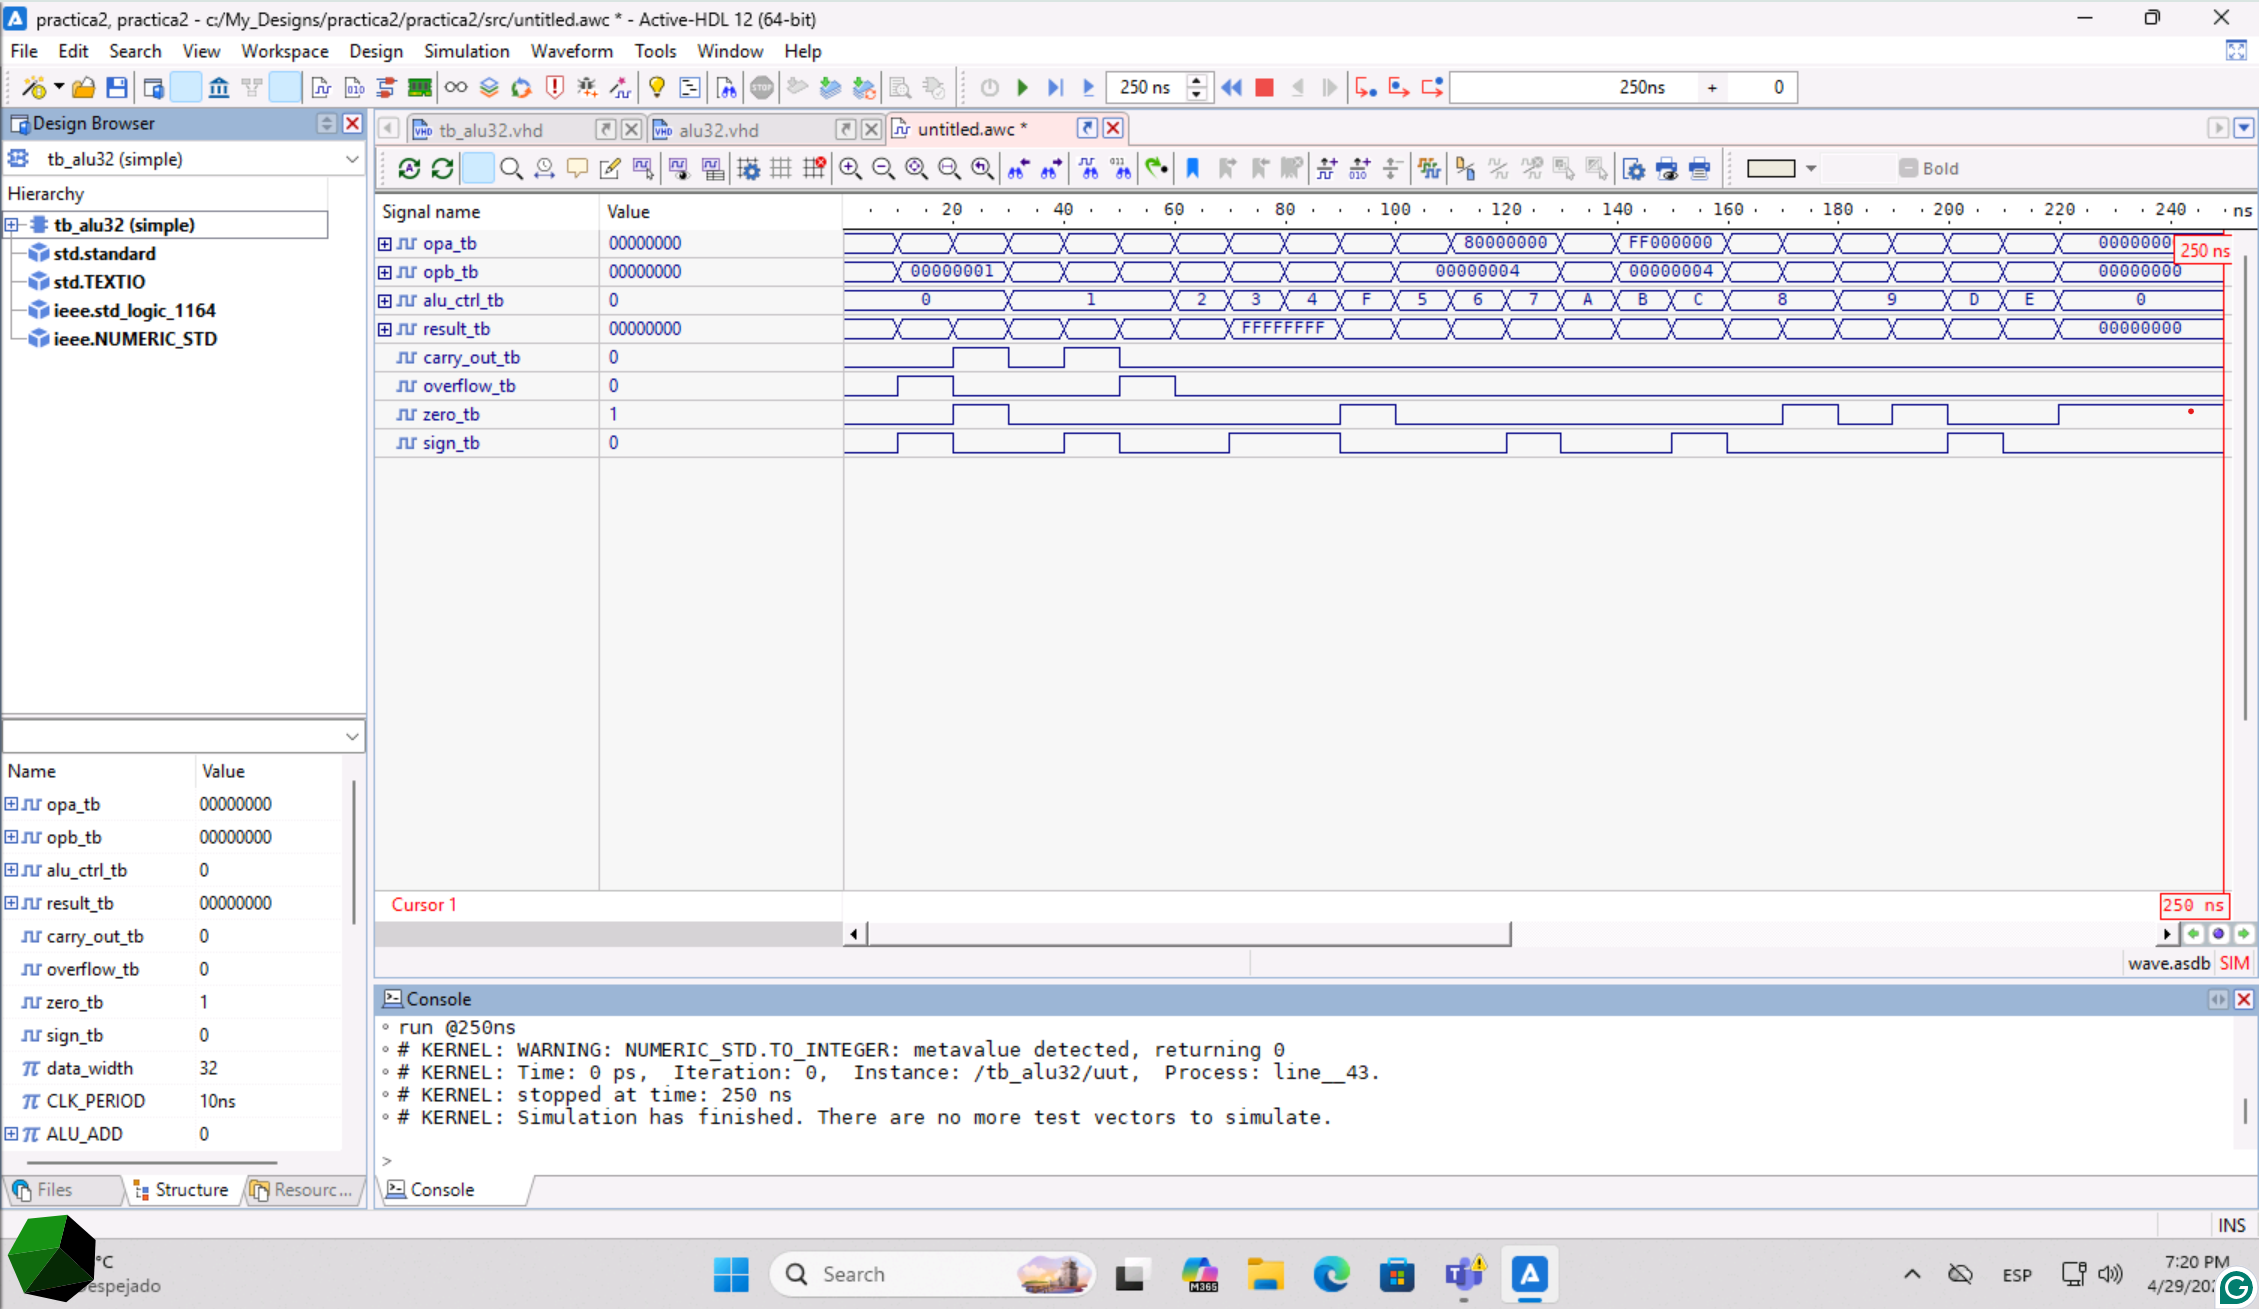
\includegraphics[width=\textwidth]{sim_general.png}
\caption{Vista panorámica de la simulación: 23 vectores ejecutados de \SI{0}{\nano\second} a \SI{230}{\nano\second}.}
\label{fig:general}
\end{figure}

\subsection{Operaciones aritméticas}
La Figura \ref{fig:arit} muestra los seis casos aritméticos. En el primer vector se realiza una suma sencilla $5 + 3 = 8$ sin activar ninguna bandera más allá de las predeterminadas. En el segundo, $\mathtt{7FFFFFFF} + 1$ produce $\mathtt{80000000}$, que en complemento a dos corresponde al mínimo entero negativo: \textit{Overflow} pasa a 1 y \textit{Sign} también, ya que el resultado tiene el bit más significativo activo. El tercer caso es un \textit{wrap-around} sin signo: $\mathtt{FFFFFFFF} + 1$ se desborda a cero, lo que activa simultáneamente \textit{CarryOut} y \textit{Zero}.

Para la resta, el caso $10 - 3$ no genera banderas extras. Cuando los operandos se invierten ($3 - 10$) el resultado en complemento a dos es $\mathtt{FFFFFFF7}$ (es decir, $-7$): \textit{Sign} se activa y \textit{CarryOut} también, ya que la condición sin signo $A < B$ se interpreta como préstamo. El último caso, $\mathtt{80000000} - 1$, ilustra el desbordamiento clásico al restar uno al mínimo negativo: el resultado pasa a ser positivo ($\mathtt{7FFFFFFF}$) y \textit{Overflow} se enciende.

\begin{figure}[H]
\centering
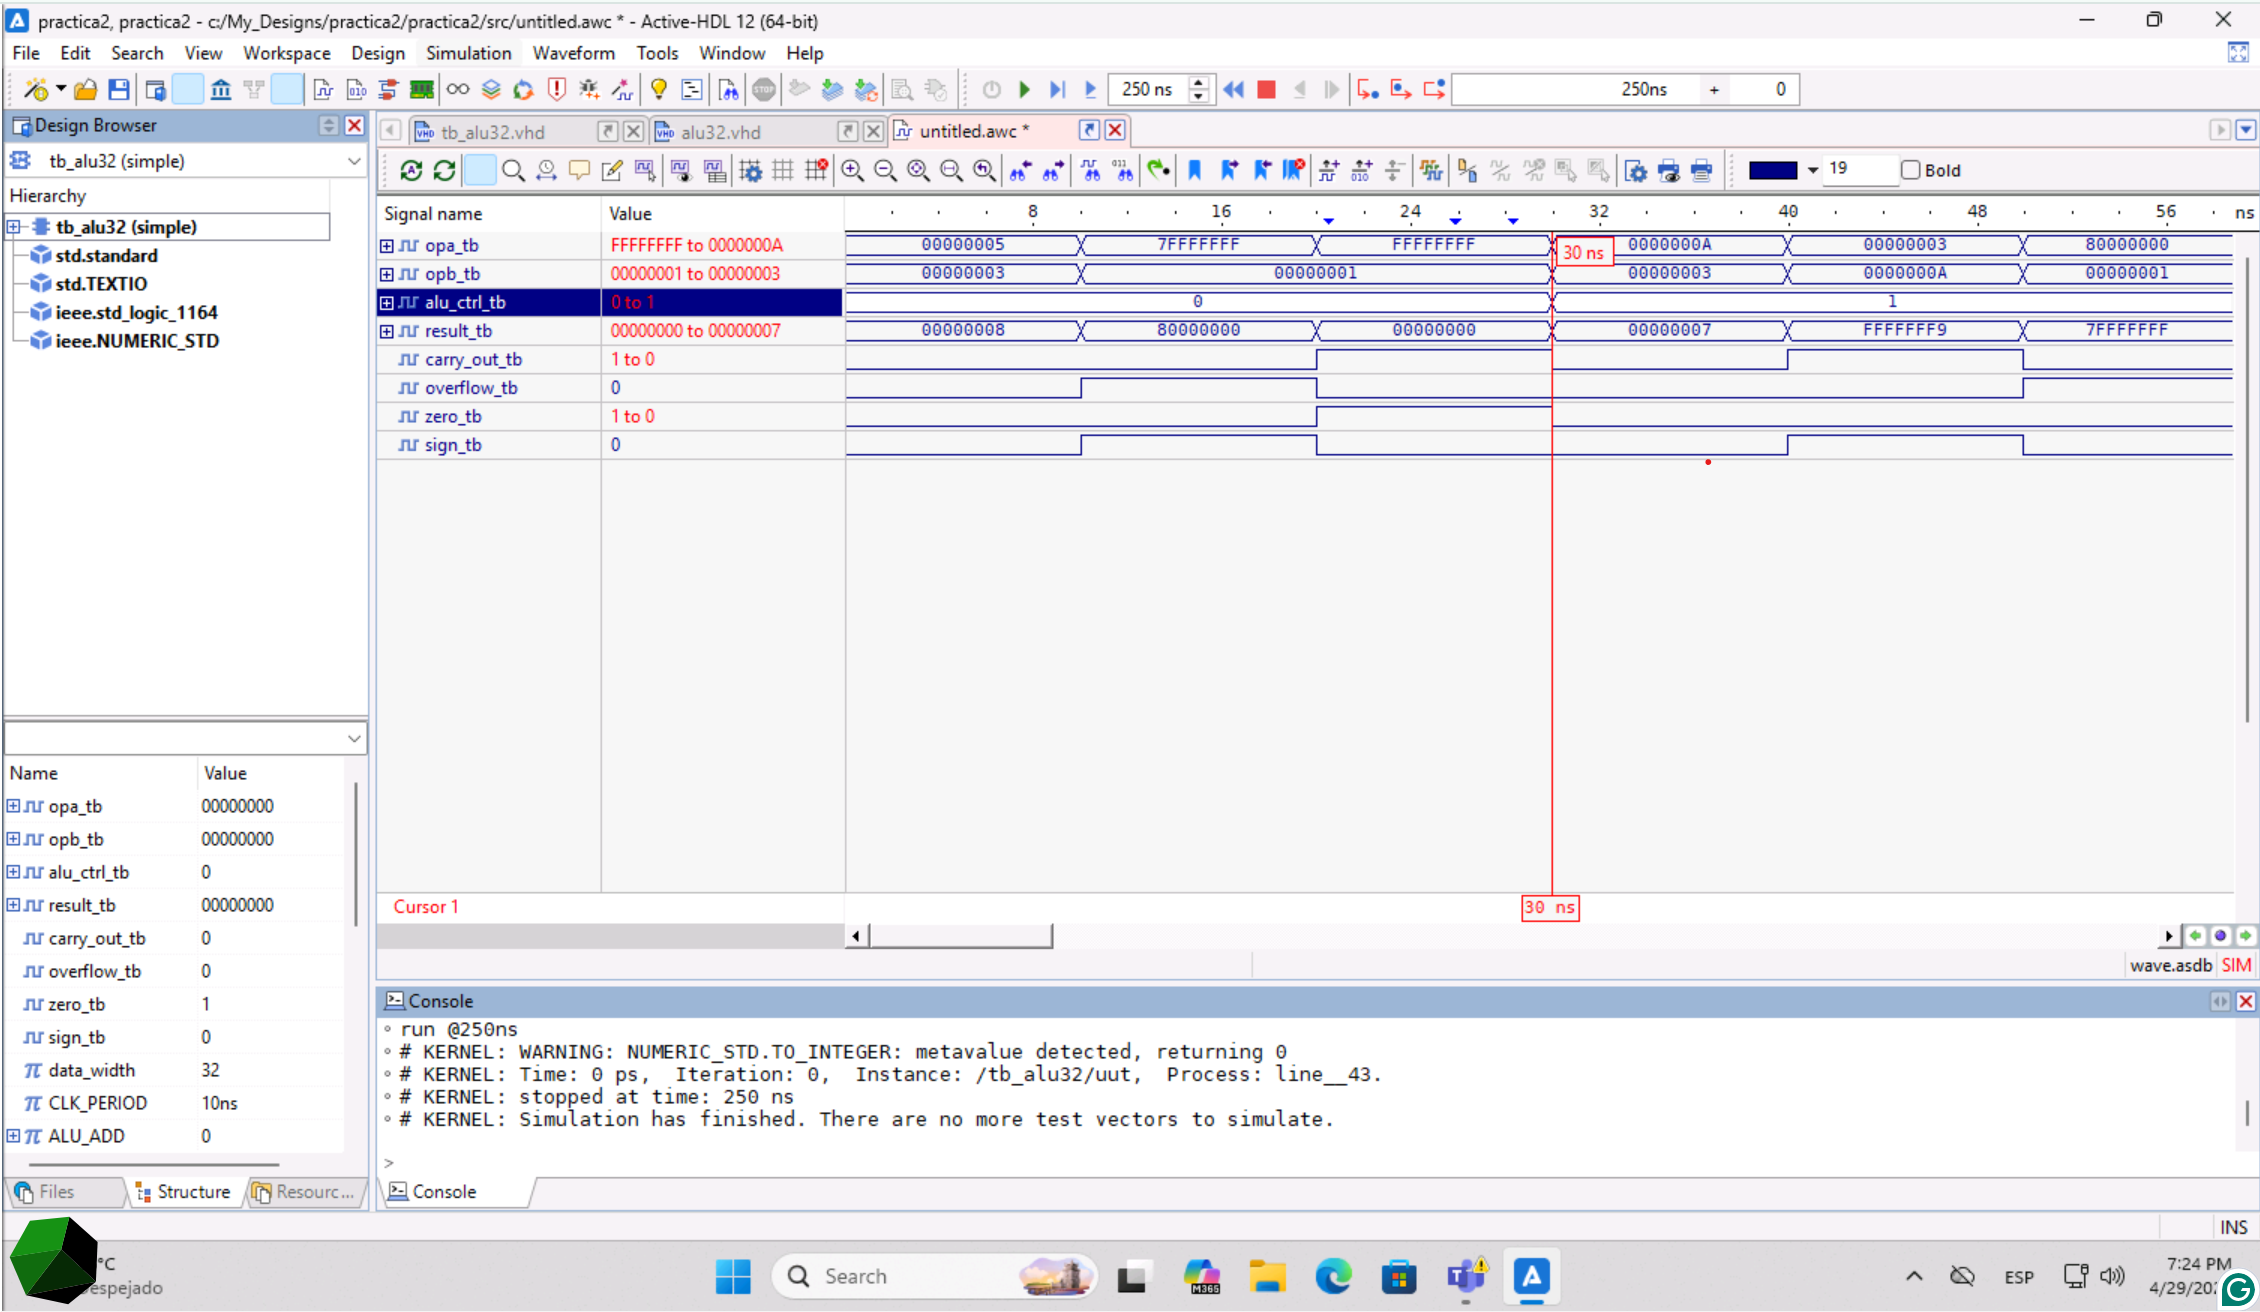
\includegraphics[width=\textwidth]{sim_aritmeticas.png}
\caption{Operaciones aritméticas \texttt{ADD} y \texttt{SUB} (\SIrange{0}{60}{\nano\second}).}
\label{fig:arit}
\end{figure}

\subsection{Operaciones lógicas}
En la Figura \ref{fig:logicas} se observan los cuatro casos lógicos. La operación \texttt{AND} entre $\mathtt{FF00FF00}$ y $\mathtt{0F0F0F0F}$ deja en cada nibble únicamente los bits comunes, dando $\mathtt{0F000F00}$. La \texttt{OR} entre dos máscaras complementarias en mitad alta y baja produce todos los bits en uno ($\mathtt{FFFFFFFF}$), con \textit{Sign} activo. La \texttt{XOR} sobre patrones $\mathtt{AAAA5555}$ y $\mathtt{5555AAAA}$ también devuelve $\mathtt{FFFFFFFF}$, ya que las posiciones de los bits están exactamente intercambiadas. Por último, la \texttt{NOR} entre $\mathtt{00FF00FF}$ y $\mathtt{FF00FF00}$ produce $\mathtt{00000000}$ porque los dos operandos cubren todas las posiciones; este caso ejercita la bandera \textit{Zero}.

\begin{figure}[H]
\centering
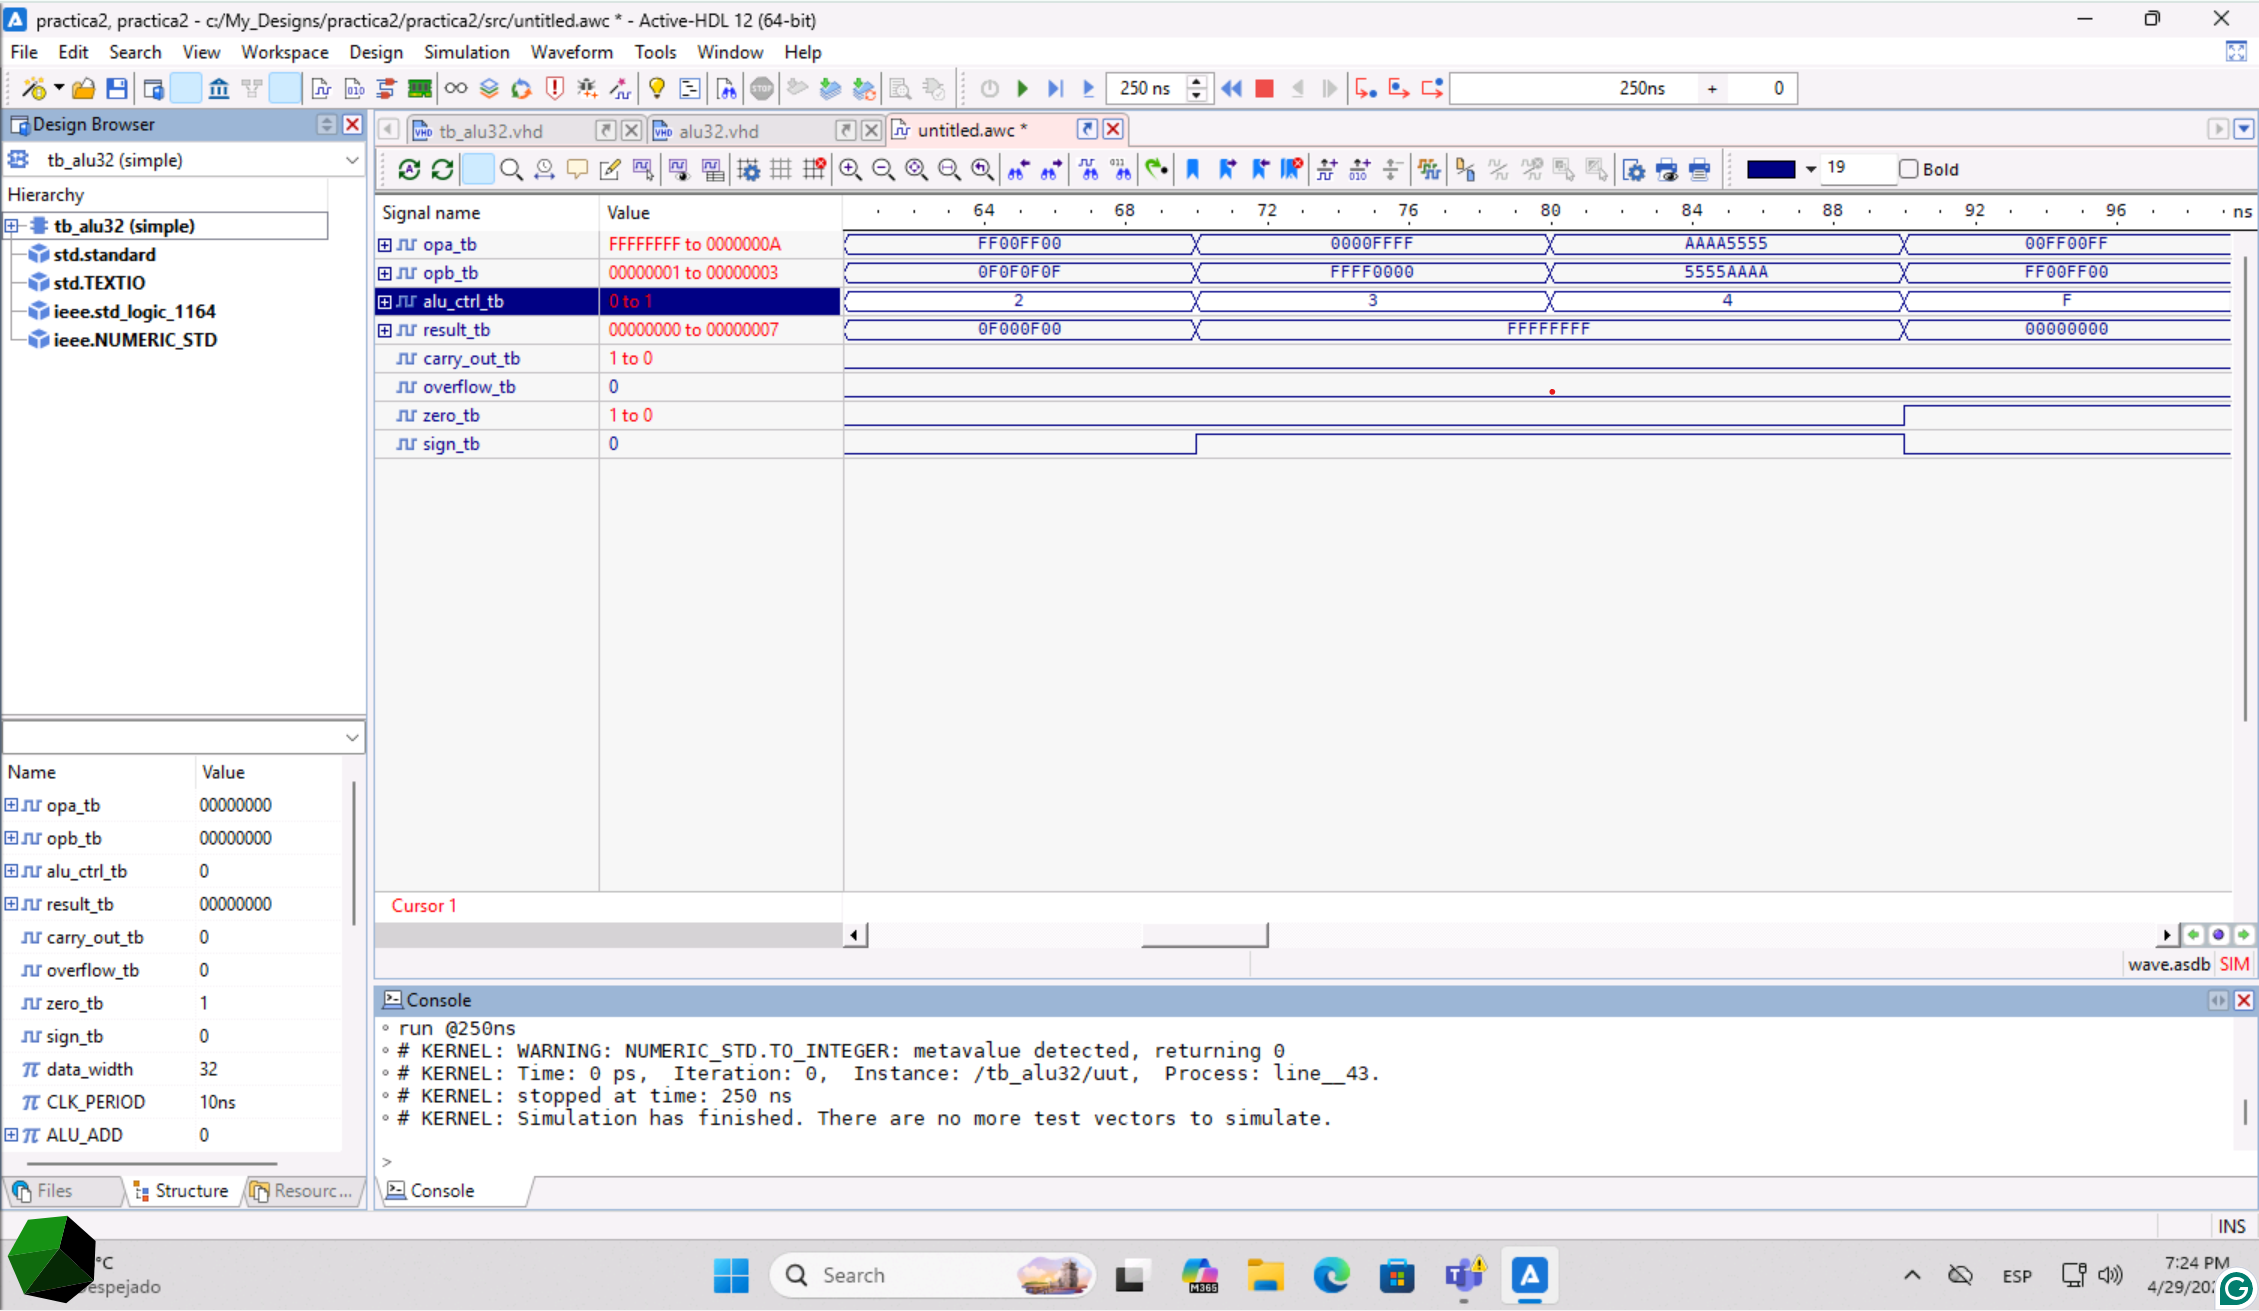
\includegraphics[width=\textwidth]{sim_logicas.png}
\caption{Operaciones lógicas \texttt{AND}, \texttt{OR}, \texttt{XOR} y \texttt{NOR} (\SIrange{60}{100}{\nano\second}).}
\label{fig:logicas}
\end{figure}

\subsection{Corrimientos por registro}
La Figura \ref{fig:corr} ilustra los tres corrimientos cuando la cantidad se toma de $B[4:0]$. Para \texttt{SLL} con $A = \mathtt{00000001}$ y un corrimiento de cuatro posiciones, el resultado es $\mathtt{00000010}$. Con $\mathtt{80000000}$ y la misma cantidad, \texttt{SRL} desplaza ceros desde la izquierda y produce $\mathtt{08000000}$, mientras que \texttt{SRA} replica el bit de signo y produce $\mathtt{F8000000}$. La diferencia entre las dos últimas operaciones es la evidencia clave del corrimiento aritmético: \texttt{SRA} preserva el signo y mantiene la bandera \textit{Sign} activa, lo cual es esperable cuando el operando es negativo.

\begin{figure}[H]
\centering
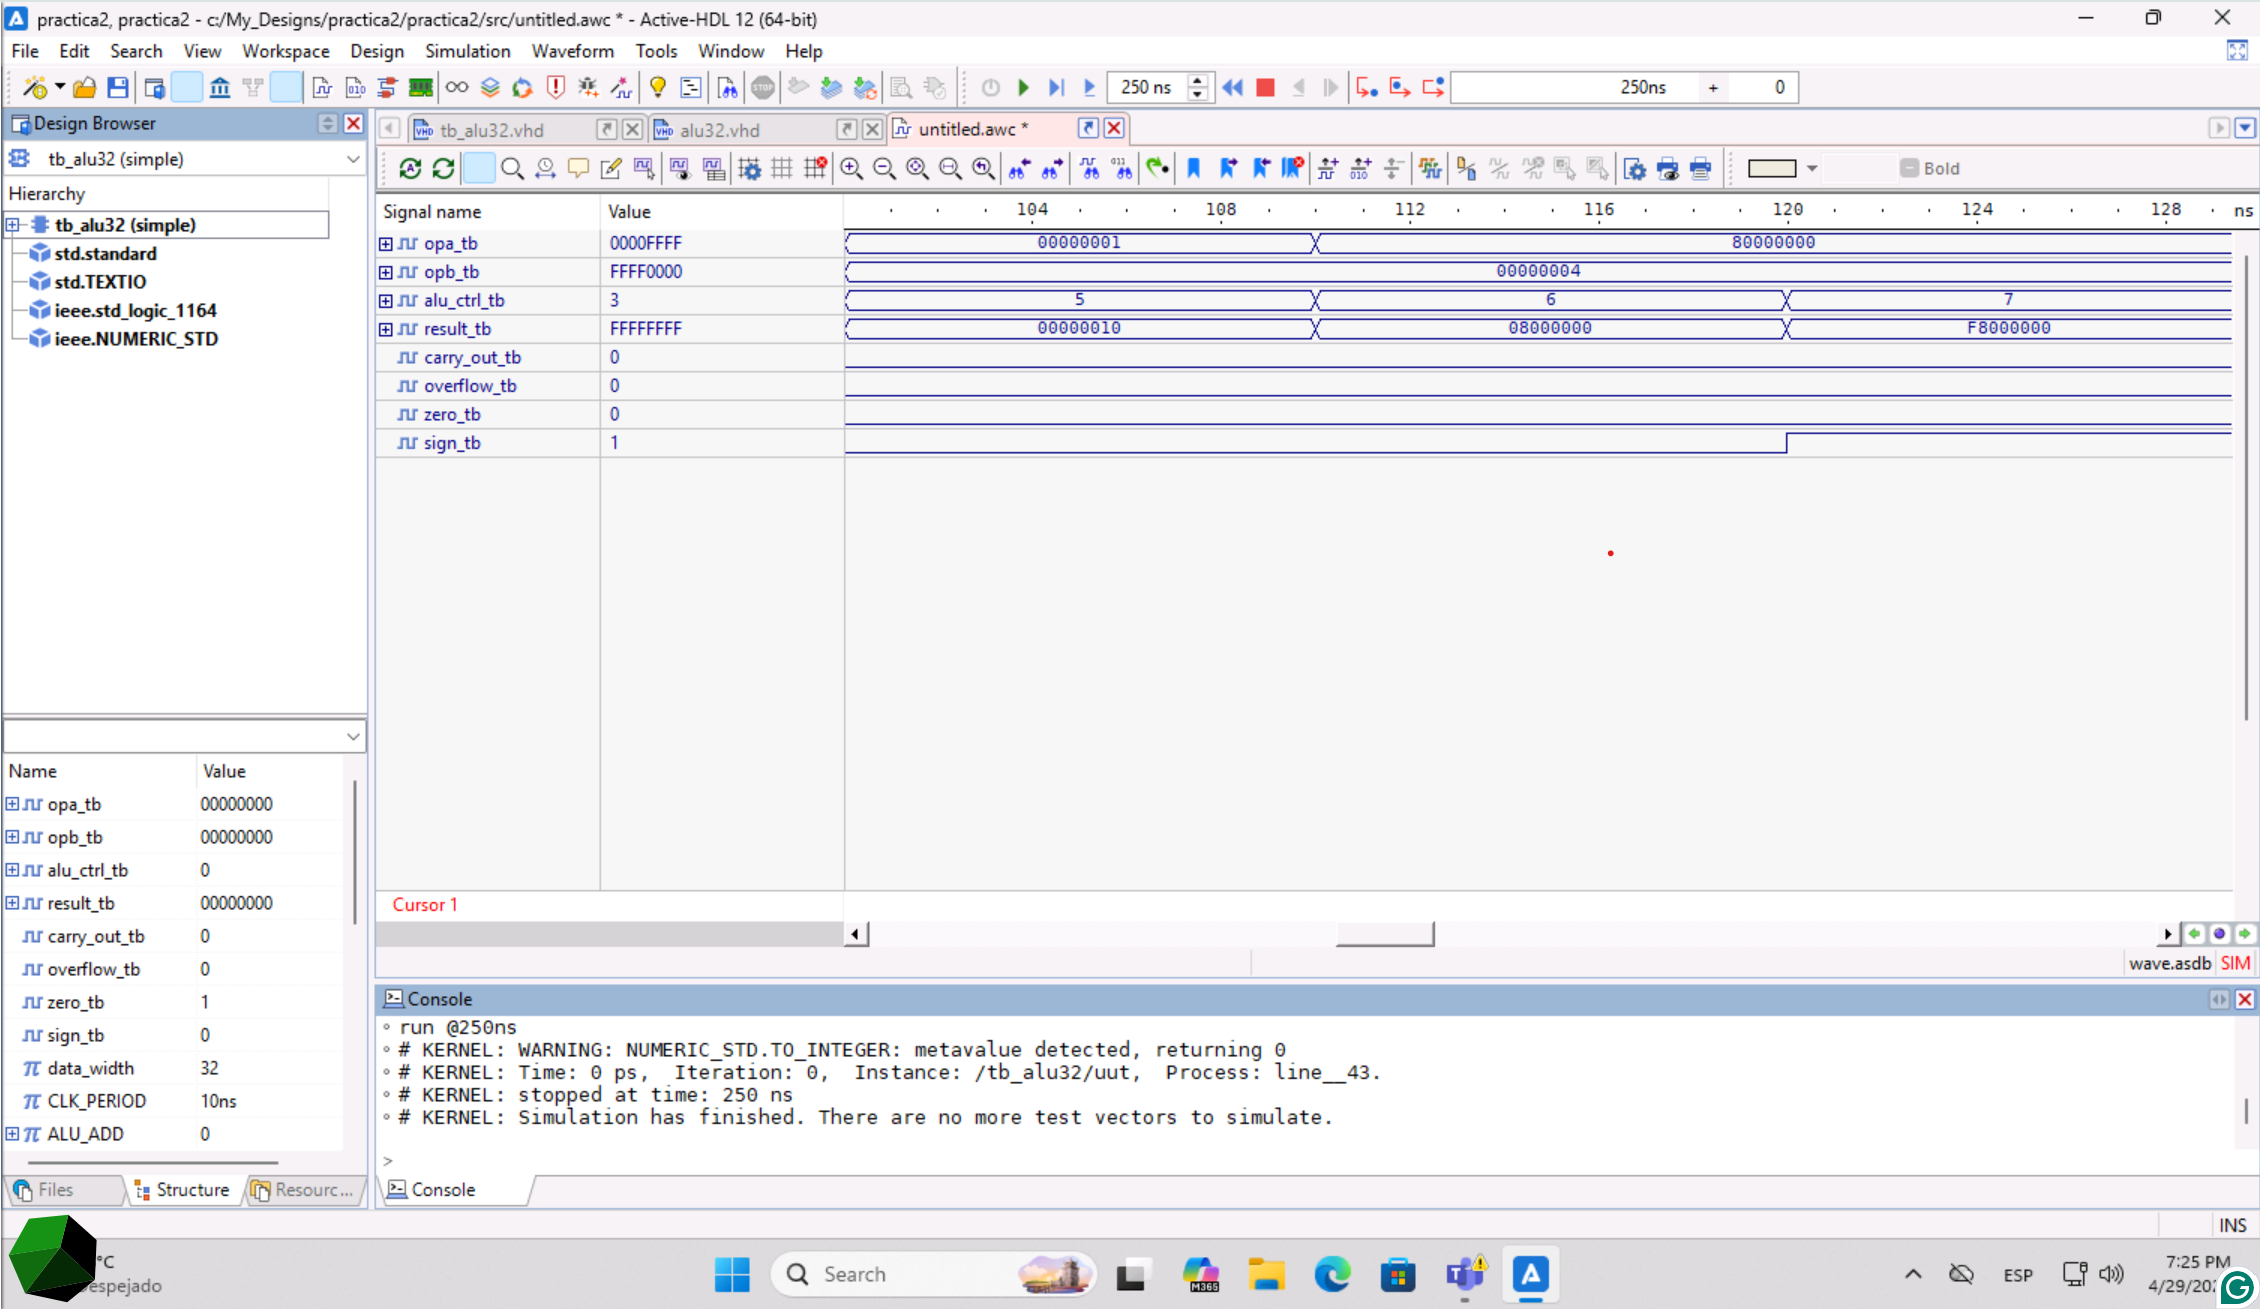
\includegraphics[width=\textwidth]{sim_corrimientos.png}
\caption{Corrimientos \texttt{SLL}, \texttt{SRL} y \texttt{SRA} (\SIrange{100}{130}{\nano\second}).}
\label{fig:corr}
\end{figure}

\subsection{Corrimientos con inmediato}
A nivel de hardware, las versiones \texttt{SLLI}, \texttt{SRLI} y \texttt{SRAI} comparten lógica con sus contrapartes; la única diferencia conceptual es el origen del operando $B$, que en el caso inmediato proviene del campo de instrucción y se trunca a cinco bits. En la Figura \ref{fig:corr_inm} se aplican $A = \mathtt{00000001}$ con desplazamiento de ocho ($\mathtt{00000100}$), y $A = \mathtt{FF000000}$ con desplazamiento de cuatro para \texttt{SRLI} ($\mathtt{0FF00000}$) y \texttt{SRAI} ($\mathtt{FFF00000}$). Nuevamente la diferencia entre las dos últimas confirma la propagación del bit de signo en el corrimiento aritmético.

\begin{figure}[H]
\centering
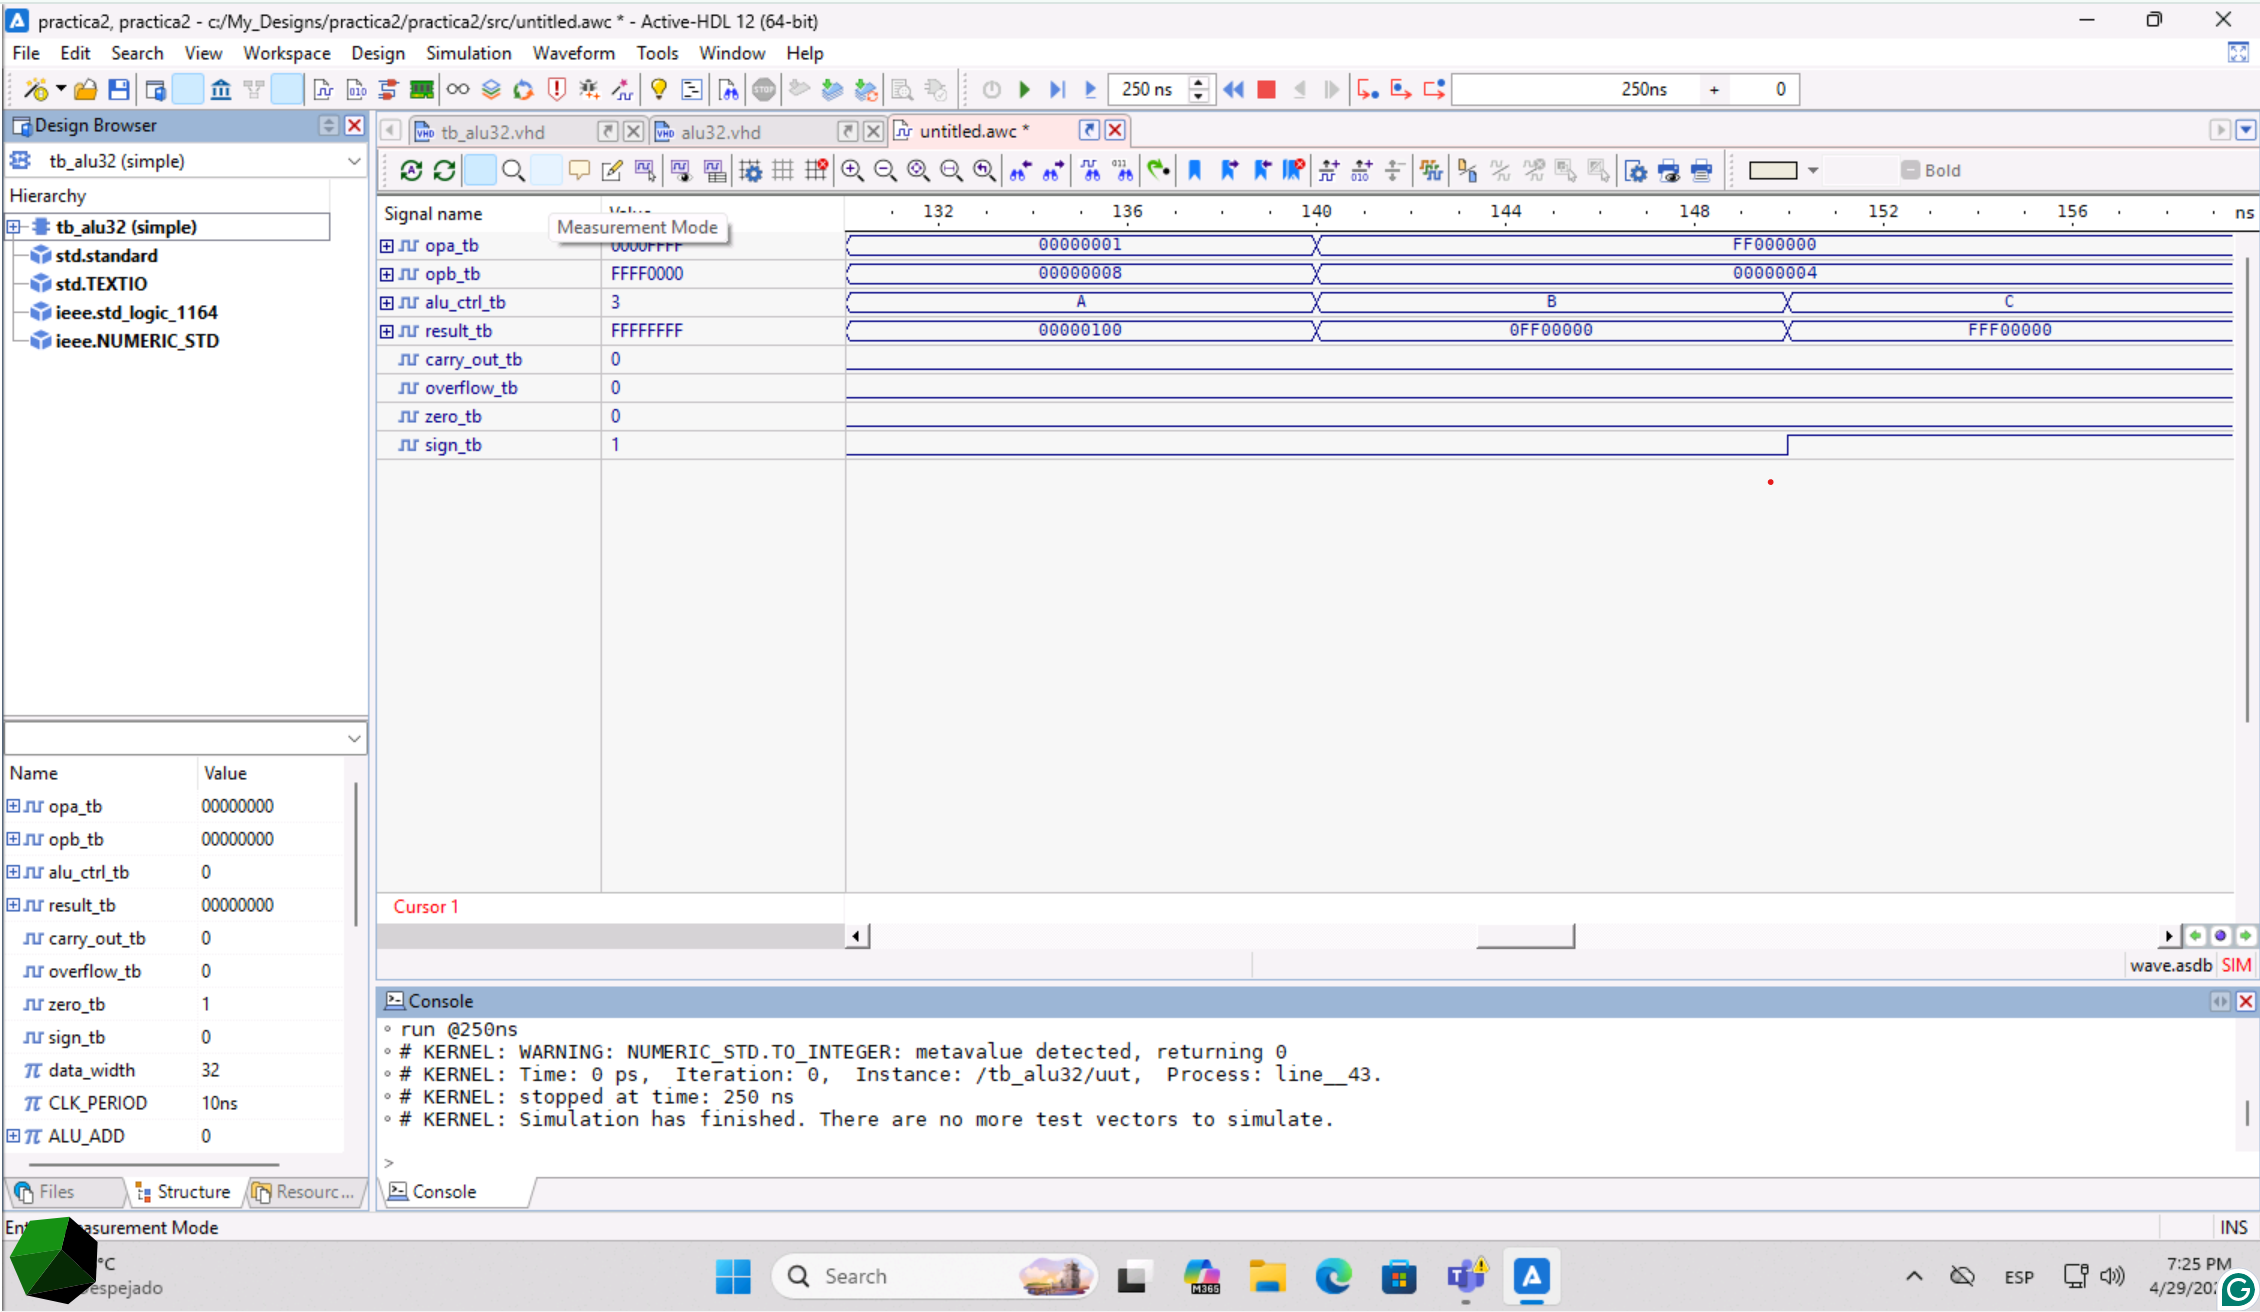
\includegraphics[width=\textwidth]{sim_corrimientos_inm.png}
\caption{Corrimientos con inmediato \texttt{SLLI}, \texttt{SRLI} y \texttt{SRAI} (\SIrange{130}{160}{\nano\second}).}
\label{fig:corr_inm}
\end{figure}

\subsection{Comparaciones}
En la Figura \ref{fig:cmp} se comparan los casos con signo y sin signo. Para \texttt{SLT}, $A = \mathtt{FFFFFFFF}$ se interpreta como $-1$ y $B = 1$ como uno positivo; al ser $-1 < 1$, el resultado es $\mathtt{00000001}$. El segundo caso, $5 < 3$, es falso y el resultado vale cero. Para \texttt{SLTU} la interpretación es sin signo: $\mathtt{00000001} < \mathtt{FFFFFFFF}$ es verdadero (uno frente al máximo no firmado), por lo que el resultado vuelve a ser $\mathtt{00000001}$; en el último caso, $5 < 3$ sin signo también es falso. La comparación entre los dos casos $A = \mathtt{FFFFFFFF}, B = 1$ resume bien la diferencia entre \texttt{SLT} y \texttt{SLTU}: el mismo par de operandos produce $1$ en la versión con signo y $0$ en la versión sin signo.

\begin{figure}[H]
\centering
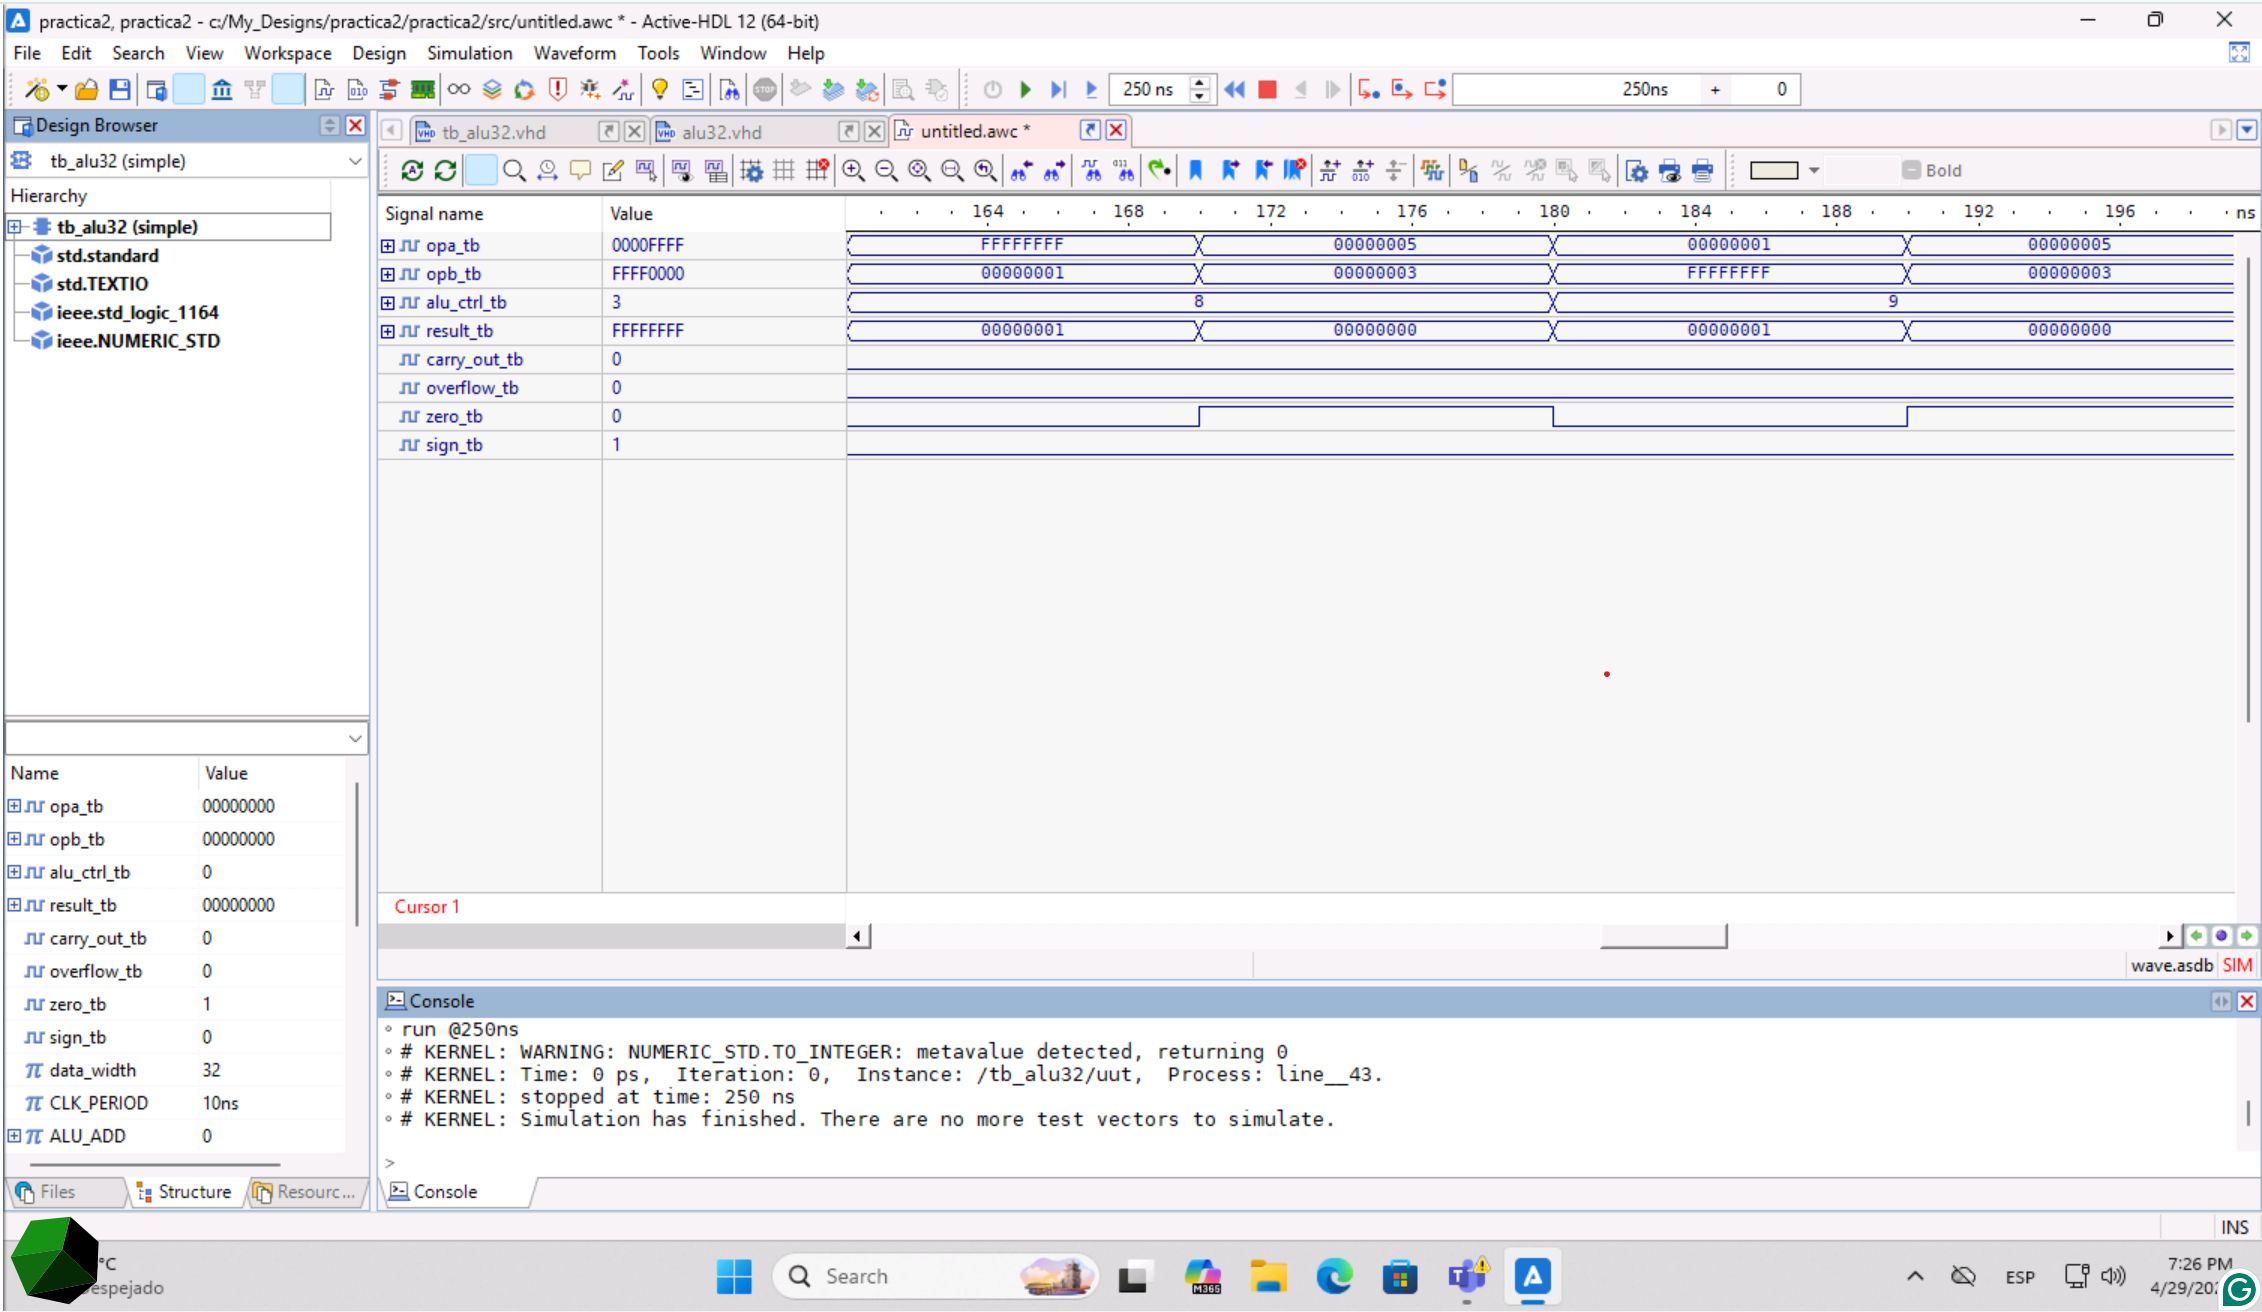
\includegraphics[width=\textwidth]{sim_comparaciones.png}
\caption{Comparaciones \texttt{SLT} y \texttt{SLTU} (\SIrange{160}{200}{\nano\second}).}
\label{fig:cmp}
\end{figure}

\subsection{LUI, AUIPC y caso de bandera \textit{Zero}}
La Figura \ref{fig:lui} cubre los últimos tres vectores. La operación \texttt{LUI} con $B = \mathtt{000ABCDE}$ desplaza $B$ doce posiciones a la izquierda y obtiene $\mathtt{ABCDE000}$, que coloca el inmediato en los 20 bits superiores del resultado. \texttt{AUIPC} suma al PC (operando $A = \mathtt{00001000}$) el inmediato $B = \mathtt{00000010}$ ya desplazado, dando $\mathtt{00011000}$. Finalmente, el último vector aplica \texttt{ADD} con ambos operandos en cero para verificar la bandera \textit{Zero}: el resultado es $\mathtt{00000000}$ y \textit{Zero} se enciende.

\begin{figure}[H]
\centering
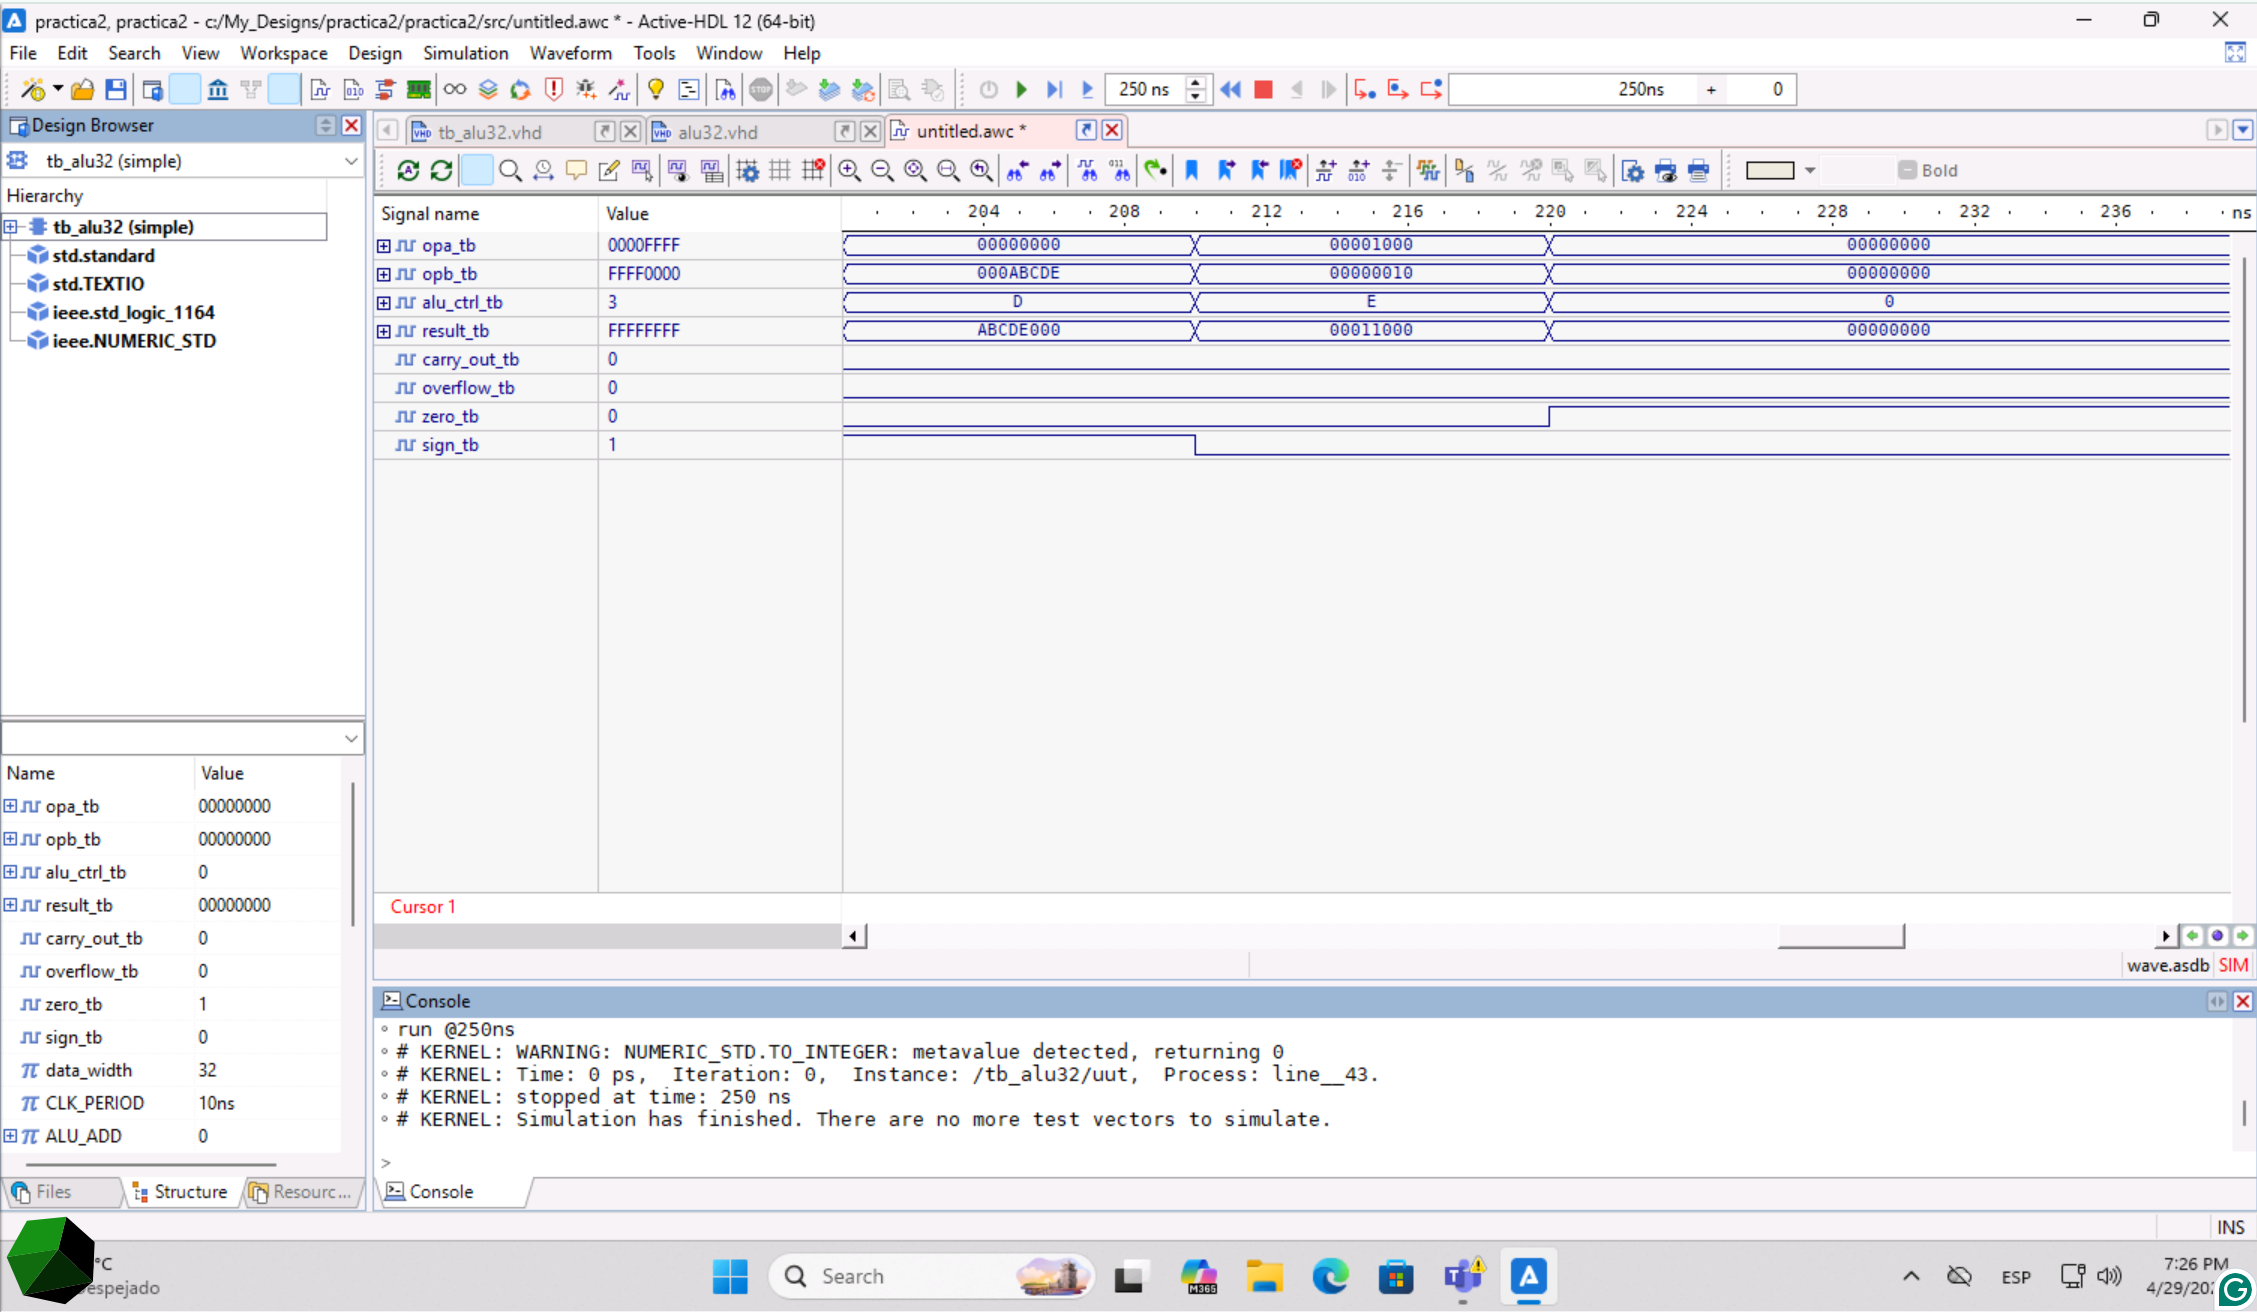
\includegraphics[width=\textwidth]{sim_lui_auipc_zero.png}
\caption{\texttt{LUI}, \texttt{AUIPC} y verificación de la bandera \textit{Zero} (\SIrange{200}{240}{\nano\second}).}
\label{fig:lui}
\end{figure}

\section{Cuestionario / Actividades complementarias}

\subsection{¿Por qué la cantidad de corrimiento usa solo $B[4:0]$?}
Porque en RV32I los registros son de 32 bits y un corrimiento mayor a 31 no tiene sentido aritmético: desplazaría todo el contenido hasta dejar solo ceros (o el bit de signo, en el caso aritmético). Cinco bits permiten codificar exactamente los valores $0$ a $31$. Tomar más bits duplicaría información sin agregar comportamiento, además de ser inconsistente con la codificación del campo inmediato en las instrucciones \texttt{SLLI}, \texttt{SRLI} y \texttt{SRAI}.

\subsection{¿Cuál es la diferencia entre \texttt{SLT} y \texttt{SLTU}?}
Ambas devuelven \texttt{0x00000001} cuando $A < B$ y \texttt{0x00000000} en caso contrario, pero la interpretación de los operandos cambia. \texttt{SLT} los toma como enteros con signo en complemento a dos, por lo que $\mathtt{FFFFFFFF}$ es $-1$ y resulta menor que cualquier número positivo. \texttt{SLTU} los interpreta sin signo, donde $\mathtt{FFFFFFFF}$ es el valor máximo posible y resulta mayor que cualquier otro operando salvo él mismo.

\subsection{¿Cómo se detecta el desbordamiento en suma y resta con signo?}
En suma, hay desbordamiento cuando los dos operandos tienen el mismo signo y el resultado tiene signo opuesto: dos positivos no pueden sumar un resultado negativo en aritmética correcta. En resta, hay desbordamiento cuando los signos de los operandos son distintos y el signo del resultado no coincide con el signo de $A$. La fórmula equivalente $\text{Overflow} = A_{31} \oplus B_{31} \oplus R_{31}$ funciona para suma; para resta hay que considerar $\sim B$ o aplicar la condición directa de signos.

\subsection{¿Por qué \texttt{LUI} usa un corrimiento de 12 posiciones?}
Porque la codificación del inmediato superior en RV32I dedica 20 bits al campo inmediato, y este valor representa los 20 bits más significativos del resultado de 32 bits. Desplazar el inmediato 12 posiciones a la izquierda lo coloca en la mitad alta y deja en cero los 12 bits inferiores, que típicamente se completan con un \texttt{ADDI} posterior para construir constantes de 32 bits.

\section{Buenas prácticas}
Durante el desarrollo se aplicaron varias prácticas que conviene mantener en futuros diseños: usar la biblioteca \texttt{numeric\_std} en lugar de \texttt{std\_logic\_arith} para que las conversiones entre \texttt{signed}, \texttt{unsigned} y \texttt{std\_logic\_vector} sean explícitas; declarar constantes simbólicas para los códigos de operación, lo cual facilita la lectura del \texttt{case}; e inicializar variables internas con valores por defecto al inicio del proceso para evitar advertencias de \textit{metavalue} durante la simulación. En el banco de pruebas se separó cada vector con un \texttt{wait for CLK\_PERIOD} para que las transiciones queden alineadas en la \textit{waveform}, lo que simplifica la inspección visual.

\section{Conclusiones}
Se implementó y verificó una ALU de 32 bits con las dieciséis operaciones de RV32I solicitadas, junto con las cuatro banderas de estado requeridas. Las simulaciones en Active-HDL coincidieron con los valores esperados de la Tabla \ref{tab:vectores} en todos los casos: las operaciones aritméticas reportaron correctamente los desbordamientos con signo y los acarreos sin signo, las lógicas dejaron las banderas aritméticas en cero y solo afectaron \textit{Zero} y \textit{Sign}, los corrimientos respetaron tanto la cantidad limitada a cinco bits como la diferencia entre extensión con cero y extensión con signo, y las comparaciones discriminaron correctamente entre interpretación con y sin signo.

La parte que requirió mayor atención fue la generación de \textit{CarryOut} y \textit{Overflow} en suma y resta. La versión inicial de la ALU dejaba ambos en cero, lo que hubiera ocultado errores en la unidad de control. Al extender los operandos a 33 bits y aplicar las reglas de signo, el comportamiento quedó alineado con la especificación. La convención de usar el operando $A$ como Program Counter en \texttt{AUIPC} mantiene la interfaz simple y evita agregar un puerto adicional.

Como trabajo futuro se propone construir un banco de pruebas auto-verificable con \texttt{assert} en cada vector, lo que permitiría detectar regresiones automáticamente al ampliar el conjunto de operaciones (por ejemplo, hacia las extensiones M y A de RISC-V) sin depender de la inspección visual de los diagramas de tiempo.

\section{Referencias}
\begin{thebibliography}{9}
\bibitem{manual_practica}
O. Guillén Fernández. \textit{Práctica 2: Unidad Aritmética Lógica (ALU) RISC-V de 32 bits}. Universidad de las Américas Puebla.

\bibitem{riscv_spec}
RISC-V International. \textit{The RISC-V Instruction Set Manual, Volume I: Unprivileged Specification}. Disponible en: \url{https://riscv.org/technical/specifications/}

\bibitem{patterson_hennessy}
D. A. Patterson y J. L. Hennessy. \textit{Computer Organization and Design RISC-V Edition: The Hardware Software Interface}. Morgan Kaufmann, 2020.

\bibitem{ieee_vhdl}
IEEE. \textit{IEEE Standard VHDL Language Reference Manual}. (Referencia general al estándar).

\bibitem{active_hdl}
Aldec. \textit{Active-HDL Documentation}. Disponible en: \url{https://www.aldec.com/en/products/fpga_simulation/active_hdl}
\end{thebibliography}

\section*{Repositorio del proyecto}
\addcontentsline{toc}{section}{Repositorio del proyecto}

El código fuente VHDL de la ALU, el banco de pruebas y las capturas de las formas de onda obtenidas en Active-HDL se encuentran disponibles en el siguiente repositorio público de GitHub:
\begin{center}
\url{https://github.com/Robbienicur/Arquitecturas-Computacionales/tree/main/Practica-2}
\end{center}
La carpeta \texttt{Practica-2} del repositorio contiene los archivos \texttt{alu32.vhd} y \texttt{tb\_alu32.vhd}, las imágenes de la simulación y este mismo reporte en formato PDF.

\end{document}
